\appendix
% \twocolumn[...] starts a new page and sets its argument across both columns, so the heading and the two
% figures stay together on one page (a figure* placed after the heading would move to the next page).
\twocolumn[{%
\section{Additional figures}\label{sec:appendix}
\vspace{2mm}
\noindent
\begin{minipage}[t]{0.48\textwidth}
\centering
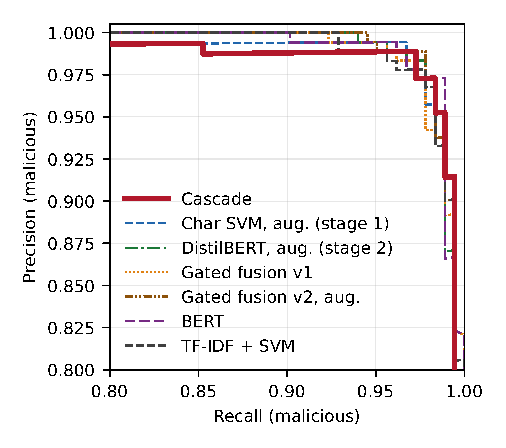
\includegraphics{figures/pr_curves}
\captionof{figure}{Precision-recall curves of the malicious class (smishing and spam against ham) on the clean three-class test set, seed 1; only the upper right corner is shown}
\label{fig:pr}
\end{minipage}\hfill
\begin{minipage}[t]{0.48\textwidth}
\centering
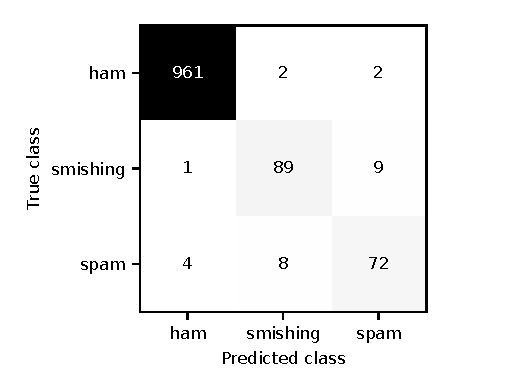
\includegraphics{figures/confusion_cascade}
\captionof{figure}{Confusion matrix of the cascade on the clean three-class test set, seed 1 (rows: true class)}
\label{fig:confusion}
\end{minipage}
\vspace{4mm}
}]
